\documentclass[11pt,a4paper]{article}

% ── Packages ──────────────────────────────────────────────────────────
\usepackage[utf8]{inputenc}
\usepackage[T1]{fontenc}
\usepackage{lmodern}
\usepackage[margin=2.5cm]{geometry}
\usepackage{amsmath,amssymb,amsthm,mathtools}
\usepackage{booktabs}
\usepackage{array}
\usepackage{enumitem}
\usepackage{fancyhdr}
\usepackage{titlesec}
\usepackage{float}
\usepackage{caption}
\usepackage{subcaption}
\usepackage{tikz}
\usepackage{pgfplots}
\usepackage{pifont}
\usepackage{xcolor}
\usepackage{hyperref}
\usepackage{tcolorbox}
\pgfplotsset{compat=1.18}
\usetikzlibrary{arrows.meta,positioning,calc,decorations.pathreplacing,
                 shapes.geometric,fit,backgrounds,matrix}

\tcbuselibrary{skins,breakable}

% ── Colors ────────────────────────────────────────────────────────────
\definecolor{mlmcolor}{RGB}{50,120,200}
\definecolor{clscolor}{RGB}{200,80,40}
\definecolor{concolor}{RGB}{40,160,60}
\definecolor{mathbg}{RGB}{245,245,255}
\definecolor{intuitionbg}{RGB}{255,250,235}
\definecolor{dialectA}{RGB}{70,130,180}
\definecolor{dialectB}{RGB}{220,80,60}
\definecolor{dialectC}{RGB}{60,170,70}
\definecolor{dialectD}{RGB}{180,100,200}

% ── Environments ──────────────────────────────────────────────────────
\newtcolorbox{mathbox}[1][]{
  colback=mathbg, colframe=blue!40!black,
  fonttitle=\bfseries, title=#1,
  breakable, enhanced
}

\newtcolorbox{intuition}[1][]{
  colback=intuitionbg, colframe=orange!60!black,
  fonttitle=\bfseries, title={Intuition: #1},
  breakable, enhanced
}

\newtcolorbox{keyidea}[1][]{
  colback=green!5!white, colframe=concolor!80!black,
  fonttitle=\bfseries, title={Key Idea: #1},
  breakable, enhanced
}

\theoremstyle{definition}
\newtheorem{definition}{Definition}[section]

\hypersetup{
    colorlinks=true,
    linkcolor=blue!70!black,
    citecolor=green!50!black,
    urlcolor=blue!60!black,
}

% ── Header ────────────────────────────────────────────────────────────
\pagestyle{fancy}
\fancyhf{}
\fancyhead[L]{\small\textit{From Zero to Dialect Geometry}}
\fancyhead[R]{\small\thepage}
\renewcommand{\headrulewidth}{0.4pt}

% ── Title ─────────────────────────────────────────────────────────────
\title{%
  \textbf{From Zero to Dialect Geometry}\\[0.3em]
  \Large A Complete Guide to How Machines Learn to\\
  Distinguish Spanish Dialects\\[0.5em]
  \large MLM, Classification, Contrastive Learning, and the\\
  EigenDialectos Architecture
}
\author{EigenDialectos Project}
\date{April 2026}

\begin{document}
\maketitle
\thispagestyle{empty}

\begin{abstract}
This document explains, from absolute first principles, how the
EigenDialectos system learns to distinguish eight varieties of Spanish.
No prior knowledge of mathematics, machine learning, or linguistics is
assumed. We build every concept from the ground up: what numbers and
vectors are, how a computer can ``learn,'' what language looks like to a
machine, and finally how three different training objectives---masked
language modeling (MLM), dialect classification (CLS), and supervised
contrastive learning (SupCon)---work together to produce a geometric
map of dialectal variation. By the end, the reader will understand not
just \emph{what} each loss function does, but \emph{why} it exists,
\emph{how} it is computed, and \emph{what} the resulting numbers mean
for the science of Spanish dialectology.
\end{abstract}

\tableofcontents
\newpage

% ======================================================================
% PART I: THE FOUNDATIONS
% ======================================================================
\part{The Foundations}

% ----------------------------------------------------------------------
\section{Numbers, Lists, and Spaces}
\label{sec:vectors}

\subsection{From single numbers to lists of numbers}

A single number tells you one thing. The temperature outside is $22$.
Your height is $1.75$. A word appears $347$ times in a book.

But the world is rarely described by a single number. To describe a
point on a map you need \emph{two} numbers: latitude and longitude. To
describe a color on a screen you need \emph{three} numbers: how much
red, how much green, how much blue.

\begin{definition}[Vector]
A \textbf{vector} is an ordered list of numbers. We write it as:
\[
\mathbf{v} = \begin{pmatrix} v_1 \\ v_2 \\ \vdots \\ v_n \end{pmatrix}
\]
The number $n$ is called the \textbf{dimension} of the vector. Each
entry $v_i$ is called a \textbf{component}.
\end{definition}

\begin{intuition}{Vectors as addresses}
Think of a vector as an address in a space with $n$ independent
directions. In two dimensions, the address $(3, 5)$ means ``go 3
steps east and 5 steps north.'' In 384 dimensions---which is what our
model uses---the address has 384 independent directions. You cannot
visualize 384 directions, but the mathematics works identically to 2.
\end{intuition}

\subsection{Distance between vectors}

If two addresses are close together, the things they describe are
similar. We need a way to measure ``closeness.''

\begin{mathbox}[Euclidean distance]
The distance between two vectors $\mathbf{a}$ and $\mathbf{b}$ in
$n$ dimensions is:
\[
d(\mathbf{a}, \mathbf{b})
= \sqrt{(a_1 - b_1)^2 + (a_2 - b_2)^2 + \cdots + (a_n - b_n)^2}
= \sqrt{\sum_{i=1}^{n} (a_i - b_i)^2}
\]
This is the Pythagorean theorem extended to $n$ dimensions.
\end{mathbox}

In two dimensions this is the straight-line distance on a map. In 384
dimensions it is exactly the same formula, just with more terms under
the square root.

\subsection{Direction: the cosine similarity}

Sometimes we care not about how far apart two vectors are, but about
whether they \emph{point in the same direction}. Two vectors can have
very different lengths but point the same way.

\begin{mathbox}[Cosine similarity]
The cosine similarity between $\mathbf{a}$ and $\mathbf{b}$ is:
\[
\cos(\theta) = \frac{\mathbf{a} \cdot \mathbf{b}}
                     {\|\mathbf{a}\| \;\|\mathbf{b}\|}
= \frac{\sum_{i=1}^n a_i \, b_i}
       {\sqrt{\sum_i a_i^2}\;\sqrt{\sum_i b_i^2}}
\]
where $\mathbf{a} \cdot \mathbf{b} = \sum_i a_i b_i$ is the
\textbf{dot product} and $\|\mathbf{a}\| = \sqrt{\sum_i a_i^2}$ is
the \textbf{length} (or \emph{norm}) of $\mathbf{a}$.
\end{mathbox}

The result is always between $-1$ and $+1$:
\begin{itemize}[nosep]
  \item $+1$: the vectors point in exactly the same direction.
  \item $\phantom{+}0$: the vectors are perpendicular (unrelated).
  \item $-1$: the vectors point in exactly opposite directions.
\end{itemize}

\begin{intuition}{Why direction matters for language}
If we represent the meaning of words as vectors, we want ``dog'' and
``puppy'' to point in similar directions (high cosine similarity),
while ``dog'' and ``airplane'' should point in unrelated directions
(cosine near zero). The \emph{direction} captures meaning; the
\emph{length} might capture something else (like word frequency). This
is why we often work with direction rather than raw distance.
\end{intuition}

\subsection{Unit vectors and normalization}

A \textbf{unit vector} is a vector whose length is exactly 1. You can
turn any nonzero vector into a unit vector by dividing each component
by the vector's length:
\[
\hat{\mathbf{a}} = \frac{\mathbf{a}}{\|\mathbf{a}\|}
\]
This operation is called \textbf{L2-normalization}. After
normalization, the cosine similarity between two unit vectors simplifies
to just their dot product:
\[
\cos(\theta) = \hat{\mathbf{a}} \cdot \hat{\mathbf{b}}
\]
This is computationally convenient and conceptually clean: every vector
lives on the surface of a high-dimensional sphere of radius~1.

% ----------------------------------------------------------------------
\section{What It Means to ``Learn''}
\label{sec:learning}

\subsection{Functions with adjustable knobs}

A \textbf{function} is a rule that takes an input and produces an
output. The function $f(x) = 2x + 3$ takes any number $x$ and
returns twice that number plus three.

Now imagine a function with \textbf{adjustable parameters}:
\[
f(x; w, b) = w \cdot x + b
\]
The semicolon separates the input ($x$) from the parameters ($w$ and
$b$). By changing $w$ and $b$, we change what the function does. If
$w=2, b=3$, it doubles and adds three. If $w=0.5, b=-1$, it halves
and subtracts one.

\begin{keyidea}{Learning = finding the right knobs}
A machine ``learns'' by adjusting its parameters so that its outputs
match what we want. We start with random parameter values and
gradually tune them. A model with millions of parameters is just a
very complicated function with millions of knobs.
\end{keyidea}

\subsection{The loss function: measuring how wrong you are}

To adjust the knobs, we need a way to measure how far the current
outputs are from the desired outputs. This measurement is called a
\textbf{loss function} (or \textbf{cost function}, or
\textbf{objective}).

\begin{definition}[Loss function]
A \textbf{loss function} $\mathcal{L}(\theta)$ is a single number
that measures how poorly a model with parameters $\theta$ is
performing on a given task. The goal of training is to make this
number as small as possible.
\end{definition}

\begin{intuition}{Loss as altitude}
Imagine you are standing on a hilly landscape. Your east--west
position is parameter $w$, your north--south position is parameter
$b$, and your altitude is the loss $\mathcal{L}$. Training is the
process of walking downhill---adjusting $w$ and $b$ to reach the
lowest point (the \emph{minimum}).
\end{intuition}

\subsection{Gradients: which way is downhill?}

If you are blindfolded on a hill, you can feel the slope under your
feet. The direction that descends most steeply is the
\textbf{gradient}.

\begin{mathbox}[Gradient]
The gradient $\nabla_\theta \mathcal{L}$ is a vector that points in
the direction of steepest \emph{increase} of $\mathcal{L}$. Each
component tells you how much $\mathcal{L}$ changes when you nudge the
corresponding parameter:
\[
\nabla_\theta \mathcal{L}
= \begin{pmatrix}
    \frac{\partial \mathcal{L}}{\partial \theta_1} \\[4pt]
    \frac{\partial \mathcal{L}}{\partial \theta_2} \\
    \vdots \\
    \frac{\partial \mathcal{L}}{\partial \theta_n}
  \end{pmatrix}
\]
The symbol $\frac{\partial \mathcal{L}}{\partial \theta_i}$ is a
\textbf{partial derivative}---it measures the rate of change of
$\mathcal{L}$ when only $\theta_i$ moves and everything else stays
fixed.
\end{mathbox}

To walk downhill, we go in the \emph{opposite} direction of the
gradient:
\[
\theta_{\text{new}} = \theta_{\text{old}} - \eta \cdot \nabla_\theta \mathcal{L}
\]
The small positive number $\eta$ is the \textbf{learning rate}---how
big a step we take. Too large and we overshoot the valley; too small
and we barely move.

This update rule is called \textbf{gradient descent}. When applied to
small random subsets (\emph{mini-batches}) of data at a time, it is
called \textbf{stochastic gradient descent} (SGD). Modern variants
like \textbf{AdamW} add momentum and adaptive step sizes, but the core
idea is the same: measure the slope, step opposite to it.

\subsection{Training loop}

The entire learning process is a loop:

\begin{enumerate}[nosep]
  \item Pick a mini-batch of examples from the training data.
  \item Run them through the model (the \textbf{forward pass}).
  \item Compute the loss.
  \item Compute the gradient of the loss with respect to every
        parameter (the \textbf{backward pass}, also called
        \emph{backpropagation}).
  \item Update every parameter by stepping opposite to its gradient.
  \item Repeat.
\end{enumerate}

One full pass through the entire dataset is called an \textbf{epoch}.
Our training runs for 10 epochs over 3.27 million documents.

% ----------------------------------------------------------------------
\section{Neural Networks: Stacking Simple Functions}
\label{sec:nn}

\subsection{A single neuron}

The simplest neural unit computes:
\[
z = \sigma\!\left(\sum_{i=1}^n w_i \, x_i + b\right)
= \sigma(\mathbf{w} \cdot \mathbf{x} + b)
\]
where $\mathbf{x}$ is the input vector, $\mathbf{w}$ are learnable
weights, $b$ is a learnable bias, and $\sigma$ is a nonlinear
\textbf{activation function}.

\begin{intuition}{Why nonlinearity?}
Without $\sigma$, stacking many layers of $\mathbf{w} \cdot \mathbf{x} + b$
collapses to a single linear function---no matter how many layers, you
could replace them all with one. The nonlinearity lets the network
represent curved, complex relationships. Common choices:
\begin{itemize}[nosep]
  \item \textbf{ReLU}: $\sigma(z) = \max(0, z)$ --- zero if negative,
        identity if positive. Simple and effective.
  \item \textbf{GELU}: a smooth approximation of ReLU, used in modern
        language models.
  \item \textbf{Sigmoid}: $\sigma(z) = 1/(1+e^{-z})$ --- squashes any
        number into $(0, 1)$.
\end{itemize}
\end{intuition}

\subsection{Layers}

A \textbf{layer} is a collection of neurons that all receive the same
input but have different weights. If we have $m$ neurons, the layer
takes an input vector of dimension $n$ and produces an output vector of
dimension $m$:
\[
\mathbf{h} = \sigma(W\mathbf{x} + \mathbf{b})
\]
where $W$ is an $m \times n$ \textbf{weight matrix} (each row is one
neuron's weights) and $\mathbf{b}$ is a bias vector of dimension $m$.

\subsection{Deep networks}

A \textbf{deep neural network} stacks multiple layers:
\[
\mathbf{x}
\xrightarrow{\text{layer 1}} \mathbf{h}_1
\xrightarrow{\text{layer 2}} \mathbf{h}_2
\xrightarrow{\;\cdots\;} \mathbf{h}_L
\xrightarrow{\text{output}} \mathbf{y}
\]
Each layer transforms its input into a new representation. The early
layers learn simple patterns; deeper layers combine them into complex
ones. The intermediate outputs $\mathbf{h}_i$ are called
\textbf{hidden states} or \textbf{representations}.

The key insight of deep learning is that we do not design these
intermediate representations---we let gradient descent discover them
by optimizing the loss function.

% ----------------------------------------------------------------------
\section{Language as Numbers: Tokens and Embeddings}
\label{sec:tokens}

\subsection{The tokenization problem}

Computers work with numbers, not letters. The first step in any
language model is to convert text into numbers.

A \textbf{tokenizer} splits text into pieces called \textbf{tokens}
and assigns each piece a unique integer ID. The pieces are not always
whole words:

\begin{center}
\texttt{"dialectolog\'{i}a"} $\;\to\;$
\texttt{["dialect", "\#\#olog", "\#\#\'{i}a"]} $\;\to\;$
\texttt{[4521, 18903, 7442]}
\end{center}

The ``\texttt{\#\#}'' prefix indicates a sub-word continuation.
BETO---the Spanish language model we use---has a vocabulary of
approximately 31,000 tokens. Every Spanish text, no matter how long,
is converted into a sequence of IDs drawn from this fixed set.

\subsection{Token embeddings: from IDs to vectors}

An integer ID is meaningless to a neural network. We need to convert
each ID into a vector that the network can process. This is done with
an \textbf{embedding table}: a matrix $E$ of size
$(\text{vocab\_size} \times d)$, where $d$ is the embedding dimension
(768 for BETO).

Looking up token ID $i$ simply means taking row $i$ of $E$:
\[
\text{embedding}(i) = E[i] \in \mathbb{R}^{768}
\]

Initially these vectors are random. Through training, tokens that
appear in similar contexts develop similar vectors---this is how the
model learns that ``perro'' and ``can'' are related.

\subsection{The sequence: from text to a matrix}

A sentence with $L$ tokens becomes a matrix of shape $(L \times 768)$:
each row is one token's vector. The entire batch of $B$ sentences
becomes a three-dimensional array (a \textbf{tensor}) of shape
$(B \times L \times 768)$.

% ----------------------------------------------------------------------
\section{Transformers and Attention}
\label{sec:transformers}

\subsection{The problem with position}

If we just look up each token's embedding independently, we lose word
order. ``The dog bit the man'' and ``the man bit the dog'' would
produce the same set of vectors, just rearranged. We need each
token's representation to \emph{know where it sits} in the sentence
and \emph{what other tokens surround it}.

\subsection{Self-attention: every word looks at every other word}

The \textbf{self-attention mechanism} is the core innovation of the
Transformer architecture (Vaswani et al., 2017). For each token, it
computes a weighted average of all other tokens' representations,
where the weights reflect how relevant each other token is.

\begin{mathbox}[Scaled dot-product attention]
Given a sequence of $L$ vectors, each token's representation is used
to compute three vectors through learned linear transformations:
\begin{align*}
\mathbf{q}_i &= W_Q \, \mathbf{h}_i \quad \text{(query: ``what am I looking for?'')} \\
\mathbf{k}_i &= W_K \, \mathbf{h}_i \quad \text{(key: ``what do I contain?'')} \\
\mathbf{v}_i &= W_V \, \mathbf{h}_i \quad \text{(value: ``what information do I provide?'')}
\end{align*}
The attention weight from token $i$ to token $j$ is:
\[
\alpha_{ij} = \frac{\exp(\mathbf{q}_i \cdot \mathbf{k}_j / \sqrt{d_k})}
                   {\sum_{\ell=1}^{L} \exp(\mathbf{q}_i \cdot \mathbf{k}_\ell / \sqrt{d_k})}
\]
This is a \textbf{softmax} over dot products. The output for token $i$ is:
\[
\text{Attention}(\mathbf{q}_i) = \sum_{j=1}^{L} \alpha_{ij} \, \mathbf{v}_j
\]
\end{mathbox}

\begin{intuition}{Attention as a spotlight}
Imagine reading the sentence ``The bank by the river was flooded.''
When processing the word ``bank,'' the attention mechanism shines a
spotlight on ``river'' and ``flooded'' to determine that this is a
river bank, not a financial institution. The spotlight intensity
($\alpha_{ij}$) is learned, not hardcoded.
\end{intuition}

\subsection{Multi-head attention}

Rather than computing one set of attention weights, the Transformer
runs $H$ independent attention ``heads'' in parallel, each with its
own $W_Q, W_K, W_V$ matrices. One head might attend to syntactic
relationships (subject--verb), another to semantic ones
(bank--river), another to positional proximity. Their outputs are
concatenated and projected back to the original dimension.

\subsection{Transformer layers}

Each Transformer layer consists of:
\begin{enumerate}[nosep]
  \item Multi-head self-attention
  \item A residual connection (add the input back to the output)
  \item Layer normalization (stabilize the numbers)
  \item A feed-forward network (two linear layers with GELU)
  \item Another residual connection and layer normalization
\end{enumerate}

BETO stacks 12 such layers. The input---a sequence of 768-dimensional
token embeddings---passes through all 12 layers, producing a final
sequence of 768-dimensional \textbf{contextualized representations}.
The word ``bank'' now has a different vector depending on whether it
appears near ``river'' or near ``money.''

\subsection{BETO: a pretrained Spanish Transformer}

BETO (\texttt{dccuchile/bert-base-spanish-wwm-cased}) was trained on
a large corpus of Spanish text using the masked language modeling
objective (which we explain in detail in Section~\ref{sec:mlm}). It
has approximately 110 million parameters and already ``knows''
Spanish grammar, semantics, and many world facts. We use it as a
starting point and \emph{adapt} it to our dialect task, rather than
training from scratch.

\subsection{LoRA: efficient adaptation}

Retraining all 110 million parameters for our task would be slow,
memory-intensive, and would risk destroying the general Spanish
knowledge BETO already has. Instead, we use
\textbf{Low-Rank Adaptation} (LoRA).

\begin{keyidea}{LoRA}
For each weight matrix $W$ in the Transformer, LoRA freezes $W$ and
adds a small trainable correction:
\[
W' = W + \Delta W = W + B \cdot A
\]
where $A$ is an $(r \times d_{\text{in}})$ matrix and $B$ is a
$(d_{\text{out}} \times r)$ matrix. The \textbf{rank} $r$ is small
(we use $r=16$). This means $\Delta W$ has only
$r \cdot (d_{\text{in}} + d_{\text{out}})$ parameters instead of
$d_{\text{in}} \cdot d_{\text{out}}$.
\end{keyidea}

We apply LoRA to six types of weight matrices in every Transformer
layer: the query, key, value, and output projections of the attention
mechanism, plus both layers of the feed-forward network. This gives us
approximately 2.7 million trainable parameters (2.4\% of the total)
while keeping the remaining 107 million frozen. The frozen parameters
preserve general Spanish; the LoRA parameters learn dialect-specific
patterns.

% ======================================================================
% PART II: THE THREE OBJECTIVES
% ======================================================================
\newpage
\part{The Three Training Objectives}

Our model simultaneously optimizes three different loss functions,
each teaching it something different. The total loss is:
\[
\mathcal{L}_{\text{total}}
= w_{\text{mlm}} \cdot \mathcal{L}_{\text{MLM}}
+ w_{\text{cls}} \cdot \mathcal{L}_{\text{CLS}}
+ w_{\text{con}} \cdot \mathcal{L}_{\text{SupCon}}
\]
where $w_{\text{mlm}}$, $w_{\text{cls}}$, and $w_{\text{con}}$ are
weights that control how much attention the optimizer pays to each
objective. We will explain each one in depth.

% ----------------------------------------------------------------------
\section{Objective 1: Masked Language Modeling (MLM)}
\label{sec:mlm}

\subsection{The idea: learning by filling in blanks}

Masked language modeling is a self-supervised learning technique
introduced by Devlin et al.\ (2018) in the BERT model. The idea is
beautifully simple:

\begin{enumerate}[nosep]
  \item Take a sentence.
  \item Randomly hide (``mask'') some of the words.
  \item Ask the model to predict what the hidden words were.
\end{enumerate}

\begin{center}
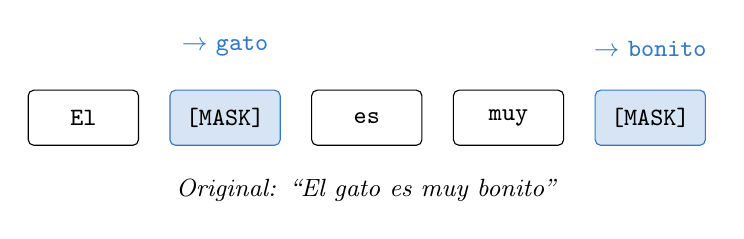
\begin{tikzpicture}[
  token/.style={draw, rounded corners=2pt, minimum height=0.7cm,
                minimum width=1.4cm, font=\small\ttfamily},
  mask/.style={token, fill=mlmcolor!20, draw=mlmcolor},
  arr/.style={-{Stealth[length=3mm]}, thick}
]
\node[token] (t1) at (0,0) {El};
\node[mask]  (t2) at (1.8,0) {[MASK]};
\node[token] (t3) at (3.6,0) {es};
\node[token] (t4) at (5.4,0) {muy};
\node[mask]  (t5) at (7.2,0) {[MASK]};

\node[font=\small, text=mlmcolor, above=0.3cm of t2] {$\to$ \texttt{gato}};
\node[font=\small, text=mlmcolor, above=0.3cm of t5] {$\to$ \texttt{bonito}};

\node[font=\small\itshape, below=0.3cm of t3]
     {Original: ``El gato es muy bonito''};
\end{tikzpicture}
\end{center}

\subsection{Why this works}

To fill in ``\texttt{[MASK]} es muy \texttt{[MASK]},'' the model must
understand grammar (the first blank is likely a noun), semantics (what
kinds of things are ``muy \emph{something}''), and context (the
surrounding words constrain the possibilities). By predicting millions
of masked words, the model builds deep representations of language.

\subsection{The mathematics: cross-entropy over a vocabulary}

At each masked position, the model outputs a vector of 31,000
numbers---one for each token in BETO's vocabulary. These numbers
(called \textbf{logits}) are raw, unnormalized scores.

\begin{mathbox}[Softmax: turning scores into probabilities]
The \textbf{softmax} function converts a vector of raw scores
$\mathbf{z} = (z_1, z_2, \ldots, z_V)$ into a probability
distribution:
\[
p_i = \frac{e^{z_i}}{\sum_{j=1}^V e^{z_j}}
\]
After softmax, all values are positive and they sum to 1. The highest
score gets the highest probability.
\end{mathbox}

Now we can measure how wrong the prediction is. If the true token is
$c$ (e.g., $c = 4521$ for ``gato''), we want $p_c$ to be as close to
1 as possible.

\begin{mathbox}[Cross-entropy loss]
\[
\mathcal{L}_{\text{CE}} = -\log(p_c)
= -\log\!\left(\frac{e^{z_c}}{\sum_{j=1}^V e^{z_j}}\right)
= -z_c + \log\!\left(\sum_{j=1}^V e^{z_j}\right)
\]
This is the \textbf{cross-entropy} between the true distribution
(all probability on class $c$) and the predicted distribution.
\end{mathbox}

\begin{intuition}{Why negative log?}
If the model assigns probability 1.0 to the correct answer:
$-\log(1.0) = 0$ (perfect, zero loss).
If it assigns probability 0.01: $-\log(0.01) = 4.6$ (high loss).
If it assigns probability 0.001: $-\log(0.001) = 6.9$ (very high).
The negative logarithm turns ``confident and correct'' into low
numbers and ``wrong'' into high numbers. It penalizes overconfident
wrong answers very harshly.
\end{intuition}

\subsection{MLM loss over a batch}

For a batch of $B$ sentences, each of length $L$, with approximately
15\% of tokens masked, the MLM loss averages across all masked positions:
\[
\mathcal{L}_{\text{MLM}} = -\frac{1}{|\mathcal{M}|}
\sum_{(i,t) \in \mathcal{M}} \log p_{c_{i,t}}
\]
where $\mathcal{M}$ is the set of all masked positions across the
batch and $c_{i,t}$ is the true token at position $t$ in sentence $i$.

\subsection{What the MLM number means}

\begin{center}
\begin{tabular}{cll}
\toprule
\textbf{MLM loss} & \textbf{Meaning} & \textbf{Interpretation} \\
\midrule
$\sim$10.3 & Random guessing & $-\log(1/31000) \approx 10.3$ \\
$\sim$7.0 & Early training & Top-1000 tokens getting mass \\
$\sim$4.0 & Good progress & Model ``understands'' grammar \\
$\sim$2.5 & Strong model & Near-human word prediction \\
$\sim$1.5 & Exceptional & Rarely achieved \\
\bottomrule
\end{tabular}
\end{center}

Our v3 run reached MLM $= 4.08$ after 3,800 optimizer steps. The
model has gone from randomly guessing among 31,000 tokens ($\text{loss}
\approx 10.3$) to effectively considering only about $e^{4.08} \approx
59$ plausible candidates per masked position. It ``knows'' Spanish
grammar and much of the vocabulary, though it still struggles with
rare words and subtle contextual cues.

\subsection{What MLM teaches the model about dialects}

MLM does not directly teach dialects---it teaches \emph{language}.
But because our corpus contains text from eight different Spanish
varieties, the model's internal representations must encode dialectal
patterns to predict masked words correctly. In a Mexican text,
``\texttt{[MASK] manejar}'' should predict ``voy a,'' while in a
Peninsular text, ``\texttt{[MASK] conducir}'' should predict
``voy a.'' To get both right, the hidden states must implicitly
represent which variety they are processing.

% ----------------------------------------------------------------------
\section{Objective 2: Dialect Classification (CLS)}
\label{sec:cls}

\subsection{The task}

Given a sentence, predict which of the eight Spanish varieties it
belongs to:

\begin{center}

\begin{tikzpicture}[
  variety/.style={draw, rounded corners=3pt, minimum width=1.2cm,
                  minimum height=0.5cm, font=\small\ttfamily}
]
\node[variety, fill=dialectA!20] (pen) at (0,0) {PEN};
\node[variety, fill=dialectB!20] (and) at (1.6,0) {AND};
\node[variety, fill=dialectC!20] (can) at (3.2,0) {CAN};
\node[variety, fill=dialectA!10] (rio) at (4.8,0) {RIO};
\node[variety, fill=dialectB!10] (mex) at (6.4,0) {MEX};
\node[variety, fill=dialectC!10] (chi) at (8.0,0) {CHI};
\node[variety, fill=dialectD!20] (car) at (9.6,0) {CAR};
\node[variety, fill=dialectD!10] (abo) at (11.4,0) {AND\_BO};
\end{tikzpicture}
\end{center}

This is a standard \textbf{multi-class classification} problem: the
model must choose one of eight categories.

\subsection{From sentence to single vector: pooling}

The Transformer produces a sequence of $L$ vectors (one per token),
but classification needs a single vector per sentence. We use
\textbf{attention pooling}: a learned weighted average that assigns
higher weight to the most informative tokens.

The result is a single 768-dimensional vector $\mathbf{p}$ that
summarizes the entire sentence.

\subsection{Standard classification}

The simplest approach is a linear classifier:
\[
\text{logits} = W_{\text{cls}} \, \mathbf{p} + \mathbf{b}_{\text{cls}}
\in \mathbb{R}^8
\]
followed by softmax and cross-entropy, exactly as in MLM but over 8
classes instead of 31,000.

This is what our v2 system used. It works, but it has a weakness: the
classifier only needs to draw \emph{hyperplanes} between classes. The
resulting representations can be arbitrarily shaped---there is no
geometric structure imposed on the embedding space.

\subsection{ArcFace: classification on a hypersphere}
\label{sec:arcface}

Our v3 system uses \textbf{ArcFace} (Deng et al., 2019), a
classification method that forces representations into a beautiful
geometric structure.

\begin{keyidea}{ArcFace: angular margin classification}
Instead of using raw dot products for classification, ArcFace:
\begin{enumerate}[nosep]
  \item Normalizes both the input vector $\mathbf{p}$ and the class
        weight vectors $\mathbf{w}_k$ to unit length.
  \item Computes cosine similarities: $\cos\theta_k = \hat{\mathbf{p}}
        \cdot \hat{\mathbf{w}}_k$.
  \item For the correct class $y$, adds an angular margin $m$:
        replaces $\cos\theta_y$ with $\cos(\theta_y + m)$.
  \item Scales by a factor $s$: the logits become $s \cdot \cos$.
\end{enumerate}
\end{keyidea}

\begin{mathbox}[ArcFace logits]
\[
\text{logit}_k =
\begin{cases}
s \cdot \cos(\theta_k + m) & \text{if } k = y \text{ (correct class)} \\
s \cdot \cos(\theta_k) & \text{if } k \neq y
\end{cases}
\]
where $\theta_k = \arccos(\hat{\mathbf{p}} \cdot \hat{\mathbf{w}}_k)$
is the angle between the input and class $k$'s prototype.

In our system: $s = 30$, $m = 0.3$ radians ($\approx 17.2°$).
\end{mathbox}

\begin{intuition}{Why the angular margin?}
Without the margin, the model only needs to push the correct class's
score slightly above the others. With the margin, the correct class
must be closer by at least $m$ radians in angular distance. This
forces the model to push each dialect's representations into tight,
well-separated angular cones on the hypersphere.
\end{intuition}

\begin{center}
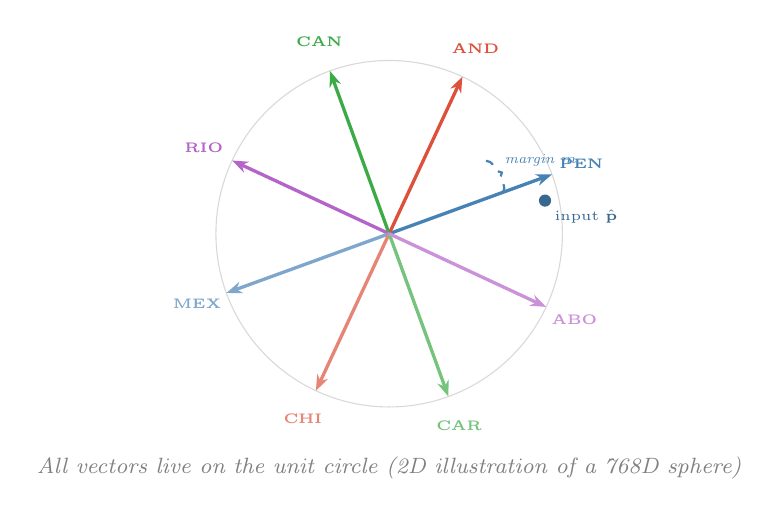
\begin{tikzpicture}[scale=2.2]
  % Unit circle
  \draw[gray!30, thin] (0,0) circle (1);

  % Class prototypes (weight vectors)
  \foreach \angle/\col/\lab in {
    20/dialectA/PEN, 65/dialectB/AND, 110/dialectC/CAN,
    155/dialectD/RIO, 200/dialectA!70/MEX, 245/dialectB!70/CHI,
    290/dialectC!70/CAR, 335/dialectD!70/ABO} {
    \draw[\col, very thick, -{Stealth[length=2mm]}]
      (0,0) -- ({cos(\angle)},{sin(\angle)});
    \node[\col, font=\tiny\bfseries] at ({1.18*cos(\angle)},{1.18*sin(\angle)}) {\lab};
  }

  % Angular margin arc for PEN
  \draw[dialectA, thick, dashed,
        decoration={brace, amplitude=3pt, mirror}, decorate]
    ({0.7*cos(20)},{0.7*sin(20)}) -- ({0.7*cos(37)},{0.7*sin(37)})
    node[midway, above right, font=\tiny\itshape, dialectA] {margin $m$};

  % Sample point
  \fill[dialectA!80!black] ({0.92*cos(12)},{0.92*sin(12)}) circle (1pt);
  \node[dialectA!80!black, font=\tiny, below right]
    at ({0.92*cos(12)},{0.92*sin(12)}) {input $\hat{\mathbf{p}}$};

  \node[font=\footnotesize\itshape, text=gray] at (0,-1.35)
    {All vectors live on the unit circle (2D illustration of a 768D sphere)};
\end{tikzpicture}
\end{center}

\subsection{Why ArcFace's CLS loss starts at 11 instead of 2}

With standard classification, the initial loss is $-\log(1/8) = \ln(8)
\approx 2.08$ (random chance among 8 classes). With ArcFace, the
scale factor $s = 30$ amplifies the logits before softmax. When the
model is untrained (random angles), the softmax outputs are more
extreme and the loss starts much higher---around 11 in our case.

This is by design. The high initial loss creates a strong gradient
signal that aggressively organizes the pooled representations into
angular cones during the early phase of training.

\subsection{What the CLS number means}

\begin{center}
\begin{tabular}{cll}
\toprule
\textbf{CLS loss} & \textbf{ArcFace meaning} & \textbf{Approximate accuracy} \\
\midrule
$\sim$11.0 & Random (untrained) & 12.5\% (chance) \\
$\sim$3.0 & Learning & $\sim$40--50\% \\
$\sim$1.3 & Good separation & $\sim$70--80\% \\
$\sim$0.5 & Strong classifier & $\sim$90--95\% \\
$\sim$0.1 & Near-perfect & $>$98\% \\
\bottomrule
\end{tabular}
\end{center}

At step 3,800, our CLS loss is 1.29. The model is already
classifying dialects well above chance, and crucially, the
768-dimensional pooled space is forming angularly separated clusters
per dialect.

\subsection{What CLS teaches the model}

Classification forces the pooled representations to encode
\emph{which dialect this is}. With ArcFace, it specifically forces
them into angularly separated cones. This provides an organized
foundation for the third objective (contrastive learning), which
operates on a projection of this space.

% ----------------------------------------------------------------------
\section{Objective 3: Supervised Contrastive Learning (SupCon)}
\label{sec:contrastive}

\subsection{The intuition: learning by comparison}

The first two objectives use \emph{labels}---the true masked word, the
true dialect. The third objective takes a fundamentally different
approach: it learns from \emph{comparisons} between examples.

\begin{keyidea}{The contrastive principle}
Given a sentence from Mexican Spanish:
\begin{itemize}[nosep]
  \item Other Mexican sentences should have \emph{similar}
        representations (\textbf{positives}).
  \item Sentences from Peninsular, Chilean, Caribbean, etc.\ Spanish
        should have \emph{different} representations
        (\textbf{negatives}).
\end{itemize}
The loss function rewards the model for making positives similar and
negatives different.
\end{keyidea}

\subsection{The projection head}

Contrastive learning does not operate directly on the 768-dimensional
pooled representations. Instead, it uses a \textbf{projection head}
that maps them into a separate 384-dimensional space:

\[
\mathbf{p} \in \mathbb{R}^{768}
\xrightarrow{\text{Linear}} \mathbb{R}^{384}
\xrightarrow{\text{BatchNorm}}
\xrightarrow{\text{ReLU}}
\xrightarrow{\text{Linear}} \mathbb{R}^{384}
\xrightarrow{\text{L2-normalize}} \hat{\mathbf{z}} \in S^{383}
\]

The output $\hat{\mathbf{z}}$ is a unit vector on the 383-dimensional
unit sphere $S^{383}$. This is the space where contrastive learning
sculpts dialect geometry.

\begin{intuition}{Why a separate projection?}
The 768-d pooled space must serve MLM and classification
simultaneously. Contrastive learning's aggressive push/pull dynamics
could distort those representations. The projection head gives
contrastive learning its own ``workspace'' without interfering with
the other two objectives. Chen et al.\ (2020) showed that this
separation is critical.
\end{intuition}

\subsection{Similarity in the projected space}

Since all projected vectors are unit-normalized, the similarity
between two sentences $i$ and $j$ is simply their dot product:
\[
\text{sim}(i, j) = \hat{\mathbf{z}}_i \cdot \hat{\mathbf{z}}_j
= \cos(\theta_{ij})
\]
This ranges from $-1$ (opposite directions) to $+1$ (same direction).

\subsection{Temperature: controlling the sharpness of similarity}

We divide the similarity by a small positive number $\tau$ called the
\textbf{temperature}:
\[
\frac{\text{sim}(i,j)}{\tau}
= \frac{\hat{\mathbf{z}}_i \cdot \hat{\mathbf{z}}_j}{\tau}
\]

\begin{intuition}{Temperature as a magnifying glass}
With $\tau = 1$, a cosine similarity of 0.7 stays 0.7. With $\tau =
0.07$ (our setting), it becomes $0.7 / 0.07 = 10$. After
exponentiation in the softmax, $e^{10} \approx 22{,}026$ while
$e^{0.7} \approx 2$. Low temperature makes the model extremely
sensitive to small differences---it forces sharper, more decisive
clustering. Think of it as turning up the ``contrast'' knob on a
photograph.
\end{intuition}

\subsection{The SupCon loss: the full formula}

For a batch of $B$ sentences, each with a dialect label, the
\textbf{supervised contrastive loss} (Khosla et al., 2020) is:

\begin{mathbox}[Supervised contrastive loss (SupCon)]
For each anchor sentence $i$ in the batch:
\[
\mathcal{L}_i = -\frac{1}{|P(i)|}
\sum_{p \in P(i)}
\log \frac{
  \exp(\hat{\mathbf{z}}_i \cdot \hat{\mathbf{z}}_p / \tau)
}{
  \displaystyle\sum_{n \in N(i)} \exp(\hat{\mathbf{z}}_i \cdot \hat{\mathbf{z}}_n / \tau)
}
\]
where:
\begin{itemize}[nosep]
  \item $P(i) = \{j \neq i : \text{label}_j = \text{label}_i\}$ ---
        the \textbf{positive set} (same dialect, different sentence).
  \item $N(i) = \{j \neq i : \text{label}_j \neq \text{label}_i\}$ ---
        the \textbf{negative set} (different dialect).
  \item The average over positives ensures the loss is not biased by the
        number of positives.
\end{itemize}
The total contrastive loss is:
\[
\mathcal{L}_{\text{SupCon}} = \frac{1}{B} \sum_{i=1}^{B} \mathcal{L}_i
\]
\end{mathbox}

\subsection{Decoupled contrastive learning (DCL)}

In the standard SupCon formula, the denominator sums over
\emph{all} non-self examples (both positives and negatives). Yeh
et al.\ (2022) showed that including positives in the denominator
creates a subtle problem: as the positive set grows, the denominator
grows too, which counteracts the attraction gradient.

\textbf{Decoupled Contrastive Learning} (DCL) removes positives from
the denominator:

\begin{mathbox}[DCL modification]
\[
\mathcal{L}_i^{\text{DCL}} = -\frac{1}{|P(i)|}
\sum_{p \in P(i)}
\log \frac{
  \exp(\hat{\mathbf{z}}_i \cdot \hat{\mathbf{z}}_p / \tau)
}{
  \displaystyle\sum_{\mathclap{n \in N(i)}}
  \exp(\hat{\mathbf{z}}_i \cdot \hat{\mathbf{z}}_n / \tau)
}
\]
The only change: the denominator sums over $N(i)$ (negatives only)
instead of all non-self examples. This \emph{decouples} the
attraction to positives from the repulsion from negatives, giving the
optimizer cleaner gradients.
\end{mathbox}

\subsection{What the gradients actually do}

Let us unpack what optimizing this loss function causes:

\begin{enumerate}
\item \textbf{Numerator gradient:} for each positive pair $(i, p)$,
  the gradient pushes $\hat{\mathbf{z}}_i$ and $\hat{\mathbf{z}}_p$
  \emph{closer} together on the sphere. Mexican sentences attract
  other Mexican sentences.

\item \textbf{Denominator gradient:} for each negative pair $(i, n)$,
  the gradient pushes $\hat{\mathbf{z}}_i$ and $\hat{\mathbf{z}}_n$
  \emph{apart}. Mexican sentences repel Chilean, Peninsular,
  Caribbean, etc.\ sentences.

\item \textbf{Hard negatives dominate:} because of the exponential
  and low temperature, negatives that are currently close to the
  anchor (high $\hat{\mathbf{z}}_i \cdot \hat{\mathbf{z}}_n$) produce
  much larger gradients. The model focuses its effort on the most
  confusable dialect pairs.
\end{enumerate}

\begin{center}
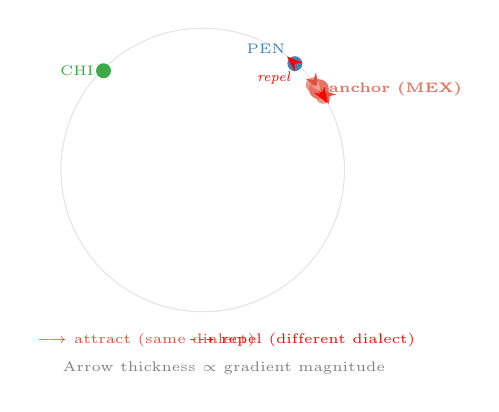
\begin{tikzpicture}[scale=1.8]
  \draw[gray!20, thin] (0,0) circle (1);

  % MEX cluster
  \fill[dialectB!60] (0.85,0.52) circle (1.5pt);
  \fill[dialectB!60] (0.78,0.60) circle (1.5pt);
  \fill[dialectB!80] (0.82,0.57) circle (2pt)
    node[right, font=\tiny\bfseries] {anchor (MEX)};

  % Draw attraction arrows
  \draw[dialectB, thick, -{Stealth[length=2mm]}, shorten >=3pt]
    (0.82,0.57) -- (0.85,0.52);
  \draw[dialectB, thick, -{Stealth[length=2mm]}, shorten >=3pt]
    (0.82,0.57) -- (0.78,0.60);

  % PEN cluster (nearby = hard negative)
  \fill[dialectA] (0.65,0.75) circle (1.5pt)
    node[above left, font=\tiny] {PEN};

  % Draw repulsion
  \draw[red, thick, -{Stealth[length=2mm]}, dashed, shorten >=3pt]
    (0.82,0.57) -- (0.91,0.42);
  \draw[red, thick, -{Stealth[length=2mm]}, dashed, shorten >=3pt]
    (0.65,0.75) -- (0.55,0.84);
  \node[red, font=\tiny\itshape] at (0.5,0.65) {repel};

  % CHI (far = easy negative, small arrow)
  \fill[dialectC] (-0.7,0.7) circle (1.5pt)
    node[left, font=\tiny] {CHI};

  \draw[red!40, thin, -{Stealth[length=1.5mm]}, dashed, shorten >=3pt]
    (0.82,0.57) -- (0.87,0.50);

  % Legend
  \node[font=\tiny, dialectB] at (-0.4,-1.2) {$\longrightarrow$ attract (same dialect)};
  \node[font=\tiny, red] at (0.7,-1.2) {$\dashrightarrow$ repel (different dialect)};
  \node[font=\tiny, gray] at (0.15,-1.4) {Arrow thickness $\propto$ gradient magnitude};
\end{tikzpicture}
\end{center}

\subsection{Cross-Batch Memory (XBM): seeing more negatives}

A single batch contains only 32 sentences (4 per dialect). That means
each anchor sees only 4 positives and 24 negatives. For contrastive
learning to work well, we want \emph{many} negatives.

\textbf{Cross-Batch Memory} (XBM; Wang et al., 2020) is a FIFO
(first-in, first-out) queue that stores projected embeddings from
recent batches:

\begin{mathbox}[XBM queue]
After each batch:
\begin{enumerate}[nosep]
  \item Compute projected embeddings $\hat{\mathbf{z}}_1, \ldots,
        \hat{\mathbf{z}}_B$ and their labels.
  \item Enqueue them into a fixed-size buffer (size 4,096 in our
        system).
  \item The oldest entries are overwritten (FIFO).
\end{enumerate}
During the next batch, the contrastive loss treats the queue entries
as additional candidates:
\begin{itemize}[nosep]
  \item \textbf{Candidates} = current batch (32) $\cup$ queue (4,096)
        = 4,128 vectors.
  \item \textbf{Anchors} = current batch only (32) --- these carry
        gradients.
  \item Queue entries are \textbf{detached} --- they do not receive
        gradients (they are ``stale'' snapshots from past steps).
\end{itemize}
\end{mathbox}

\begin{intuition}{XBM as institutional memory}
Imagine a student (the anchor) trying to learn what makes Mexican
Spanish distinctive. Without XBM, they compare against 24 examples
from other dialects. With XBM, they compare against 4,096 examples---a
much richer landscape of ``what Mexican is not.'' The examples are
slightly outdated (from previous batches), but this staleness is
harmless because the model changes slowly between steps.
\end{intuition}

\subsection{Why SupCon matters for EigenDialectos}

MLM teaches language. CLS teaches dialect identity. SupCon teaches
\textbf{dialect geometry}---the relative spatial arrangement of all
eight varieties.

The downstream analysis pipeline treats the 384-dimensional projected
embeddings as points in a geometric space and applies:
\begin{itemize}[nosep]
  \item \textbf{Spectral decomposition:} finding the principal axes of
        variation between dialects (eigenvectors of the difference
        matrices).
  \item \textbf{Procrustes alignment:} rotating and reflecting the
        per-dialect spaces so that shared vocabulary words align,
        making cross-dialect comparison possible.
  \item \textbf{Fisher scoring:} identifying which words are most
        distinctive per dialect.
\end{itemize}

For this analysis to work, the projected embeddings must capture
genuine dialectal structure---not just ``which dialect is this
sentence'' (that is CLS's job) but ``how does this dialect relate
geometrically to the others.'' Contrastive learning creates this
structure by continuously pushing and pulling dialect clusters into a
configuration that reflects their true similarities and differences.

\subsection{What the contrastive loss number means}

\begin{center}
\begin{tabular}{cll}
\toprule
\textbf{SupCon loss} & \textbf{Meaning} & \textbf{Geometric interpretation} \\
\midrule
$\sim$3.5--4.0 & Random / collapsed & All dialects overlapping \\
$\sim$2.5--3.0 & Beginning to separate & Clusters forming, high overlap \\
$\sim$1.5--2.0 & Good separation & Clear per-dialect regions \\
$\sim$0.5--1.0 & Tight clustering & Well-separated, compact clusters \\
$<$0.5 & Excellent & Dialects geometrically distinct \\
\bottomrule
\end{tabular}
\end{center}

In the current v3 run, contrastive loss is 0.0 because we are in the
pretrain phase (epochs 1--2), where it is intentionally disabled. When
it activates at epoch 3, we expect it to start around 3.0--3.5 and
drop rapidly thanks to the geometric foundation that ArcFace has
already built.

The v2 system's contrastive loss was stuck at 7.92 for the entire
training run---a catastrophic failure that motivated the 13
architectural interventions in v3.

% ======================================================================
% PART III: THE FULL ARCHITECTURE
% ======================================================================
\newpage
\part{The Full Architecture}

% ----------------------------------------------------------------------
\section{Multi-Task Learning: Three Objectives, One Model}
\label{sec:multitask}

\subsection{Why three objectives at once?}

Each objective teaches something the others cannot:

\begin{center}
\renewcommand{\arraystretch}{1.4}
\begin{tabular}{>{\bfseries}l p{5cm} p{5cm}}
\toprule
\textbf{Objective} & \textbf{What it teaches} & \textbf{What it cannot teach} \\
\midrule
\textcolor{mlmcolor}{MLM} &
  Grammar, vocabulary, semantics. Builds rich 768-d hidden states
  that encode what words mean in context. &
  No dialect awareness. Treats all Spanish identically. \\
\textcolor{clscolor}{CLS} &
  Which dialect a sentence belongs to. Organizes the 768-d pooled
  space into angularly separated cones (via ArcFace). &
  No geometric structure beyond ``which class.'' Does not capture
  relative relationships between dialects. \\
\textcolor{concolor}{SupCon} &
  Dialect geometry. Sculpts the 384-d projection space so that
  intra-dialect distances are small and inter-dialect distances are
  large. Captures relative dialect relationships. &
  No language understanding. Operates on projected vectors, not raw
  token representations. Needs MLM and CLS to provide a good
  foundation. \\
\bottomrule
\end{tabular}
\end{center}

\subsection{The information flow}

The following diagram shows how data flows through the model during
training:

\begin{center}
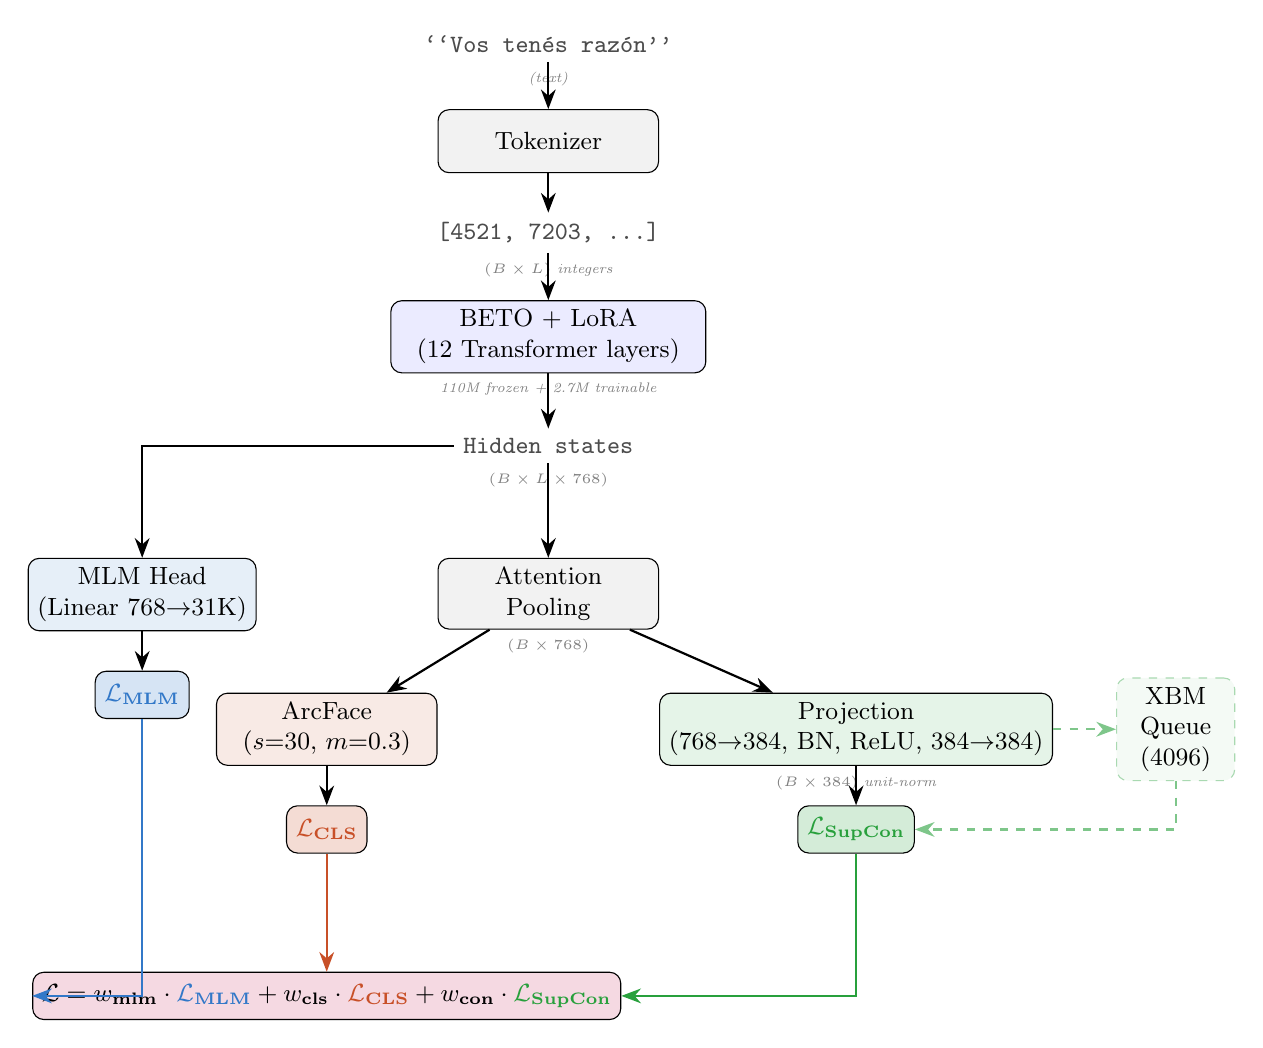
\begin{tikzpicture}[
  block/.style={draw, rounded corners=4pt, minimum height=0.8cm,
                minimum width=2.8cm, font=\small, align=center},
  data/.style={font=\small\ttfamily, text=gray!60!black},
  loss/.style={draw, rounded corners=4pt, minimum height=0.6cm,
               font=\small\bfseries},
  arr/.style={-{Stealth[length=2.5mm]}, thick},
  dim/.style={font=\tiny\itshape, text=gray}
]

% Input
\node[data] (input) at (0,0) {``Vos ten\'es raz\'on''};
\node[dim, below=0pt of input] {(text)};

% Tokenizer
\node[block, fill=gray!10, below=0.6cm of input] (tok) {Tokenizer};
\draw[arr] (input) -- (tok);

% Token IDs
\node[data, below=0.5cm of tok] (ids) {[4521, 7203, ...]};
\node[dim, below=0pt of ids] {$(B \times L)$ integers};
\draw[arr] (tok) -- (ids);

% BETO + LoRA
\node[block, fill=blue!8, below=0.6cm of ids,
      minimum width=4cm] (beto) {BETO + LoRA\\(12 Transformer layers)};
\node[dim, below=0pt of beto] {110M frozen + 2.7M trainable};
\draw[arr] (ids) -- (beto);

% Hidden states
\node[data, below=0.7cm of beto] (hidden) {Hidden states};
\node[dim, below=0pt of hidden] {$(B \times L \times 768)$};
\draw[arr] (beto) -- (hidden);

% Three branches
% MLM branch
\node[block, fill=mlmcolor!12, below left=1.2cm and 2.5cm of hidden]
     (mlmhead) {MLM Head\\(Linear 768$\to$31K)};
\node[loss, fill=mlmcolor!20, below=0.5cm of mlmhead] (mlmloss)
     {\textcolor{mlmcolor}{$\mathcal{L}_{\text{MLM}}$}};
\draw[arr] (hidden) -| (mlmhead);
\draw[arr] (mlmhead) -- (mlmloss);

% Pooling (center)
\node[block, fill=gray!10, below=1.2cm of hidden]
     (pool) {Attention\\Pooling};
\node[dim, below=0pt of pool] {$(B \times 768)$};
\draw[arr] (hidden) -- (pool);

% CLS branch
\node[block, fill=clscolor!12, below left=0.8cm and 0cm of pool]
     (arcface) {ArcFace\\($s{=}30$, $m{=}0.3$)};
\node[loss, fill=clscolor!20, below=0.5cm of arcface] (clsloss)
     {\textcolor{clscolor}{$\mathcal{L}_{\text{CLS}}$}};
\draw[arr] (pool) -- (arcface);
\draw[arr] (arcface) -- (clsloss);

% Projection branch
\node[block, fill=concolor!12, below right=0.8cm and 0cm of pool]
     (proj) {Projection\\(768$\to$384, BN, ReLU, 384$\to$384)};
\node[dim, below=0pt of proj] {$(B \times 384)$ unit-norm};
\draw[arr] (pool) -- (proj);

% SupCon loss
\node[loss, fill=concolor!20, below=0.5cm of proj] (conloss)
     {\textcolor{concolor}{$\mathcal{L}_{\text{SupCon}}$}};
\draw[arr] (proj) -- (conloss);

% XBM
\node[block, fill=concolor!5, draw=concolor!40, dashed,
      right=0.8cm of proj, minimum width=1.5cm] (xbm) {XBM\\Queue\\(4096)};
\draw[arr, concolor!60, dashed] (proj) -- (xbm);
\draw[arr, concolor!60, dashed] (xbm) |- (conloss);

% Total loss
\node[loss, fill=purple!15, below=1.5cm of clsloss,
      minimum width=5.5cm] (total)
     {$\mathcal{L} = w_{\text{mlm}} \cdot
       \textcolor{mlmcolor}{\mathcal{L}_{\text{MLM}}} +
       w_{\text{cls}} \cdot
       \textcolor{clscolor}{\mathcal{L}_{\text{CLS}}} +
       w_{\text{con}} \cdot
       \textcolor{concolor}{\mathcal{L}_{\text{SupCon}}}$};
\draw[arr, mlmcolor] (mlmloss) |- (total);
\draw[arr, clscolor] (clsloss) -- (total);
\draw[arr, concolor] (conloss) |- (total);

\end{tikzpicture}
\end{center}

\subsection{The weight curriculum}

Not all objectives are equally important throughout training. We use a
\textbf{curriculum} that changes the weights over time:

\begin{center}
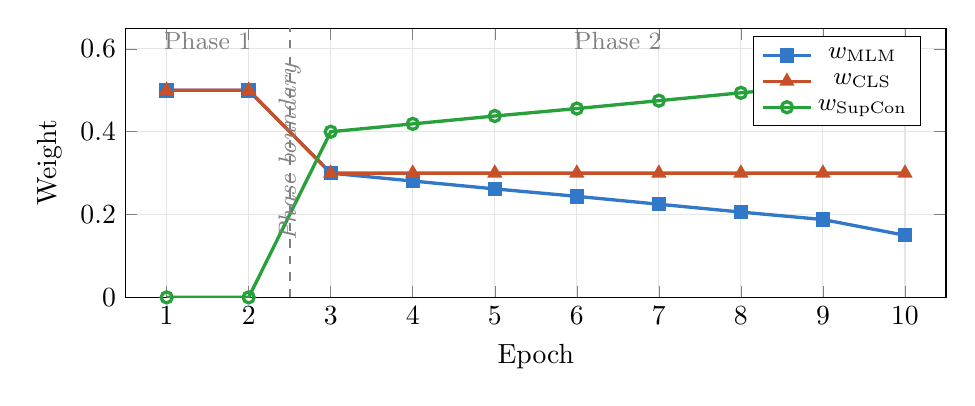
\begin{tikzpicture}
\begin{axis}[
  width=12cm, height=5cm,
  xlabel={Epoch}, ylabel={Weight},
  xmin=0.5, xmax=10.5,
  ymin=0, ymax=0.65,
  legend pos=north east,
  legend style={font=\small},
  grid=major,
  grid style={gray!20},
]
% Phase 1: pretrain (epochs 1-2)
\addplot[mlmcolor, very thick, mark=square*, mark size=2pt]
  coordinates {(1,0.5) (2,0.5) (3,0.3) (4,0.281) (5,0.262)
               (6,0.244) (7,0.225) (8,0.206) (9,0.188) (10,0.15)};
\addlegendentry{$w_{\text{MLM}}$}

\addplot[clscolor, very thick, mark=triangle*, mark size=2pt]
  coordinates {(1,0.5) (2,0.5) (3,0.3) (4,0.3) (5,0.3)
               (6,0.3) (7,0.3) (8,0.3) (9,0.3) (10,0.3)};
\addlegendentry{$w_{\text{CLS}}$}

\addplot[concolor, very thick, mark=o, mark size=2pt]
  coordinates {(1,0.0) (2,0.0) (3,0.4) (4,0.419) (5,0.438)
               (6,0.456) (7,0.475) (8,0.494) (9,0.512) (10,0.55)};
\addlegendentry{$w_{\text{SupCon}}$}

% Phase boundary
\draw[gray, dashed, thick] (axis cs:2.5,0) -- (axis cs:2.5,0.65);
\node[font=\small\itshape, text=gray, rotate=90]
  at (axis cs:2.5,0.35) {Phase boundary};
\node[font=\small, text=gray] at (axis cs:1.5,0.62) {Phase 1};
\node[font=\small, text=gray] at (axis cs:6.5,0.62) {Phase 2};
\end{axis}
\end{tikzpicture}
\end{center}

\textbf{Phase 1 (epochs 1--2):} Only MLM and CLS are active, each
with weight 0.5. The model learns language and builds an angularly
separated dialect space via ArcFace. This is the ``foundation-laying''
phase.

\textbf{Phase 2 (epochs 3--10):} SupCon activates with initial weight
0.4, gradually increasing to 0.55. MLM decreases from 0.3 to 0.15.
CLS stays at 0.3. The model now sculpts dialect geometry on top of the
foundation.

\subsection{Center loss: early contrastive assistance}

During the first 2,000 contrastive optimizer steps (early in Phase 2),
a fourth auxiliary objective called \textbf{center loss} (Wen et al.,
2016) is active:
\[
\mathcal{L}_{\text{center}} = \frac{1}{2B}
\sum_{i=1}^B \|\hat{\mathbf{z}}_i - \mathbf{c}_{y_i}\|^2
\]
where $\mathbf{c}_k$ is a learnable centroid for dialect $k$. This
simply pulls each projected embedding toward its dialect's center,
breaking the initial symmetry and giving SupCon a head start. After
2,000 steps, center loss is disabled and SupCon takes over completely.

% ----------------------------------------------------------------------
\section{The Balanced Batch Sampler}
\label{sec:sampler}

Contrastive learning requires that every batch contains examples from
all classes. If a batch happened to contain only Mexican and Chilean
sentences, the model could not learn about the other six dialects in
that step.

Our \textbf{BalancedVarietySampler} guarantees that every batch
contains exactly $k = 4$ sentences from each of the 8 varieties, for
a fixed batch size of $4 \times 8 = 32$. This ensures:
\begin{itemize}[nosep]
  \item Every anchor has at least 3 positives (same dialect) and 24
        negatives (other dialects) within the batch.
  \item With XBM, the positive/negative ratio is further enriched from
        the queue.
  \item No dialect is underrepresented in any training step.
\end{itemize}

% ----------------------------------------------------------------------
\section{From Training to Dialect Geometry}
\label{sec:geometry}

\subsection{What we extract after training}

After the model is trained, we no longer need the MLM head, the
ArcFace classifier, or the contrastive loss. We use the trained
Transformer + projection head as a feature extractor:

\begin{enumerate}[nosep]
  \item For each of the 10,800 words in our vocabulary, and for each
        of the 8 dialects:
  \item Find sentences in that dialect that contain the word.
  \item Run them through the Transformer and projection head.
  \item Average the 384-dimensional projected vectors across sentences.
  \item The result is one 384-dimensional vector per word per dialect.
\end{enumerate}

For each dialect, this produces a matrix of shape
$(10{,}800 \times 384)$: the dialect's word embedding matrix.

\subsection{Procrustes alignment}

The eight embedding matrices live in different coordinate systems
(rotated and reflected relative to each other) because the projection
was learned jointly. \textbf{Procrustes alignment} finds the best
rotation/reflection to align each dialect's space to a reference
(Peninsular Spanish), using shared ``anchor'' words that should have
similar meanings across all dialects.

After alignment, we can directly compare vectors across dialects: the
difference between the Mexican vector for ``carro'' and the Peninsular
vector for ``coche'' becomes geometrically meaningful.

\subsection{What the spectral analysis does with these embeddings}

The aligned word embeddings are the raw material for the EigenDialectos
spectral analysis:

\begin{enumerate}
  \item \textbf{Difference matrices:} for each dialect pair, compute
        $\Delta = E_A - E_B$, the word-by-word vector differences.

  \item \textbf{Eigendecomposition:} compute the principal components
        (eigenvectors) of $\Delta^\top \Delta$. The top eigenvectors
        are the ``axes of dialectal variation''---the directions in
        384-d space along which the two dialects differ most.

  \item \textbf{Fisher scoring:} project each word's difference onto
        these axes to identify which words are most distinctive per
        dialect pair.

  \item \textbf{Eigenvalue spectrum:} the eigenvalues tell us
        \emph{how much} variation exists along each axis. A steep
        spectrum (few large eigenvalues, many near-zero) means the
        dialectal differences are concentrated in a few dimensions---a
        sign of clean, structured geometry.
\end{enumerate}

This entire analysis chain requires that the contrastive loss actually
worked---that the 384-d projection space genuinely separates dialects
in a geometrically meaningful way. This is why the contrastive loss is
the most critical of the three objectives, and why its failure in v2
(stuck at 7.92) required 13 architectural interventions.

% ======================================================================
% PART IV: READING THE NUMBERS
% ======================================================================
\newpage
\part{Reading the Numbers}

% ----------------------------------------------------------------------
\section{The Training Dashboard}
\label{sec:dashboard}

During training, the system logs a line every 50 optimizer steps. Here
is a real example from the v3 run:

\begin{center}
\small\ttfamily
\begin{tabular}{rl}
epoch & 1/10 \\
step & 3800/20224 (1.88\%) \\
loss & 2.688 \\
mlm & 4.082 \\
cls & 1.294 \\
con & 0.000 \\
lr & 1.52e-04 \\
sm/s & 34.0 \\
\end{tabular}
\end{center}

Let us decode each number:

\begin{description}[style=nextline, leftmargin=2cm]
  \item[\texttt{epoch 1/10}]
    We are in epoch 1 of 10. One epoch = one full pass through 3.27
    million documents.

  \item[\texttt{step 3800/20224}]
    Optimizer step 3,800 of 20,224 in this epoch. Each step processes
    one batch of 32 sentences.

  \item[\texttt{loss = 2.688}]
    The weighted total:
    $0.5 \times 4.082 + 0.5 \times 1.294 + 0.0 \times 0.0 = 2.688$.

  \item[\texttt{mlm = 4.082}]
    The model is effectively choosing among $e^{4.082} \approx 59$
    plausible tokens per masked position. Down from 31,000 at
    initialization.

  \item[\texttt{cls = 1.294}]
    ArcFace classification loss. Down from 11.08 at initialization.
    The 768-d space is forming angularly separated dialect cones.

  \item[\texttt{con = 0.000}]
    Contrastive loss is disabled (Phase 1). Will activate at epoch 3.

  \item[\texttt{lr = 1.52e-04}]
    Current learning rate, warming up toward the target of $2
    \times 10^{-4}$.

  \item[\texttt{sm/s = 34.0}]
    Throughput: 34 samples per second on Apple Silicon MPS.
\end{description}

% ----------------------------------------------------------------------
\section{Comparative Analysis: v1 vs.\ v2 vs.\ v3}
\label{sec:comparison}

\begin{center}
\renewcommand{\arraystretch}{1.3}
\begin{tabular}{l ccc}
\toprule
& \textbf{v1 (GRL)} & \textbf{v2 (SupCon)} & \textbf{v3 (13 int.)} \\
\midrule
Contrastive method & InfoNCE + GRL & SupCon + DCL + XBM & SupCon + DCL + XBM \\
Classifier & Linear & Linear & ArcFace ($s$=30, $m$=0.3) \\
Projection & LN + GELU & LN + GELU & BN + ReLU (2-layer) \\
Projection dim & 256 & 384 & 384 \\
LoRA targets & 3 (QKV) & 6 (QKV+FFN) & 6 (QKV+FFN) \\
Max length & 128 & 256 & 256 \\
Two-phase training & No & No & Yes (2 pretrain epochs) \\
Center loss & No & No & Yes (2000 steps) \\
PCA init & No & No & Yes \\
\midrule
\multicolumn{4}{l}{\textit{At step 3800:}} \\
MLM loss & 7.64 & 5.53 & \textbf{4.08} \\
CLS loss & 9.26 & 1.63 & \textbf{1.29} \\
Contrastive & 3.78 (stuck) & 7.92 (stuck) & 0.0 (disabled, Phase 1) \\
\bottomrule
\end{tabular}
\end{center}

The critical test for v3 comes at epoch 3, when contrastive activates.
The hypothesis is that ArcFace + center loss will have built a
sufficiently organized 768-d space that the projected embeddings start
with meaningful dialect structure, allowing SupCon to descend
immediately rather than stalling.

% ----------------------------------------------------------------------
\section{What to Expect}
\label{sec:expectations}

Based on the training dynamics observed so far and the architectural
design:

\begin{center}
\renewcommand{\arraystretch}{1.3}
\begin{tabular}{l ccc l}
\toprule
\textbf{Milestone} & \textbf{MLM} & \textbf{CLS} & \textbf{SupCon}
& \textbf{What it means} \\
\midrule
End epoch 1 & $\sim$3.2 & $\sim$0.8 & 0.0 &
  Foundation complete \\
End epoch 2 & $\sim$2.8 & $\sim$0.5 & 0.0 &
  Dialect cones well-formed \\
Epoch 3, step 500 & $\sim$2.7 & $\sim$0.5 & $<$3.0 &
  \textbf{Critical: SupCon descending?} \\
Epoch 3, step 2000 & $\sim$2.6 & $\sim$0.5 & $<$2.0 &
  Phase transition confirmed \\
End epoch 5 & $\sim$2.3 & $\sim$0.4 & $<$1.0 &
  Strong dialect geometry \\
End epoch 10 & $\sim$2.0 & $\sim$0.3 & $<$0.5 &
  Mature embeddings \\
\bottomrule
\end{tabular}
\end{center}

\subsection{The critical checkpoint: epoch 3}

The single most important moment in the entire training run is when
the contrastive loss activates at epoch 3 (approximately 42 hours
from launch). There are three possible outcomes:

\begin{enumerate}
  \item \textbf{Immediate descent} (SupCon $< 2.5$ within 500 steps):
    The ArcFace preconditioning worked. The projected embeddings
    already have enough dialect structure for SupCon to find gradient
    signal. The training will succeed.

  \item \textbf{Slow descent} (SupCon $\sim$ 2.5--3.0 at step 500, then
    gradually declining): Center loss is doing its job but the
    projection head needs more time to organize. The training will
    likely succeed but may need more epochs.

  \item \textbf{Stagnation} (SupCon $> 3.0$ after 1,000 steps): The
    interventions were insufficient. This would require investigation
    and possibly a v4 design.
\end{enumerate}

% ======================================================================
% PART V: GLOSSARY
% ======================================================================
\newpage
\part*{Glossary}
\addcontentsline{toc}{part}{Glossary}

\begin{description}[style=nextline, leftmargin=3.5cm, font=\bfseries]

  \item[Activation function]
    A nonlinear function applied after a linear transformation in a
    neural network. Common examples: ReLU, GELU, sigmoid. Without it,
    stacking layers would collapse to a single linear function.

  \item[ArcFace]
    A classification method that adds an angular margin penalty to
    force representations into well-separated angular cones on a
    hypersphere. Used in our CLS objective.

  \item[Attention]
    A mechanism that allows each token in a sequence to ``look at''
    every other token and compute a weighted average of their
    representations, where the weights reflect relevance.

  \item[Backpropagation]
    The algorithm for computing gradients of the loss with respect to
    every parameter in a neural network. Works by applying the chain
    rule of calculus backwards through the network.

  \item[Batch]
    A small subset of the training data processed together in one
    forward/backward pass. Our batch size is 32 (4 sentences
    $\times$ 8 dialects).

  \item[BatchNorm]
    Batch Normalization. Normalizes activations \emph{across} the
    batch dimension. Preserves inter-sample variance, which is
    important for contrastive learning.

  \item[BETO]
    A pretrained Spanish Transformer model
    (\texttt{bert-base-spanish-wwm-cased}) with 110M parameters,
    trained on a large Spanish corpus. Our starting point.

  \item[Center loss]
    An auxiliary loss that pulls embeddings toward learnable class
    centroids. Used during the first 2,000 contrastive steps to break
    initial symmetry.

  \item[Contrastive learning]
    A family of methods that learn representations by comparing
    examples: pulling similar examples together and pushing different
    examples apart.

  \item[Cross-entropy]
    A loss function for classification: $-\log(p_c)$ where $p_c$ is
    the predicted probability of the correct class. Lower is better.

  \item[DCL]
    Decoupled Contrastive Learning. A variant that removes positives
    from the denominator, decoupling attraction from repulsion.

  \item[Embedding]
    A vector representation of a discrete object (token, word,
    sentence). Transforms symbolic data into continuous geometry.

  \item[Epoch]
    One complete pass through the entire training dataset.

  \item[Gradient]
    A vector of partial derivatives indicating the direction of
    steepest increase of a function. Training goes opposite to the
    gradient (downhill).

  \item[Hidden state]
    The intermediate vector representation of a token or sentence
    inside the neural network. Not directly observed; discovered
    through training.

  \item[L2-normalization]
    Dividing a vector by its length to produce a unit vector (length =
    1). All points then live on the unit sphere.

  \item[Learning rate]
    The step size in gradient descent. Too large: unstable. Too small:
    slow. Our target is $2 \times 10^{-4}$.

  \item[LoRA]
    Low-Rank Adaptation. A parameter-efficient method that adds small
    trainable matrices to a frozen pretrained model, avoiding the cost
    and risk of full fine-tuning.

  \item[Loss function]
    A scalar that measures how poorly the model is performing. Training
    minimizes this number.

  \item[MLM]
    Masked Language Modeling. A self-supervised objective: randomly
    mask tokens and predict them. Teaches language understanding.

  \item[Projection head]
    A small neural network that maps from the Transformer's output
    space (768-d) to the contrastive space (384-d). Gives SupCon its
    own workspace without distorting the shared representations.

  \item[Softmax]
    A function that converts a vector of real numbers into a
    probability distribution (all positive, sum to 1).

  \item[SupCon]
    Supervised Contrastive Learning. Uses class labels to define
    positive (same class) and negative (different class) pairs.

  \item[Temperature]
    A scaling factor that controls the sharpness of the similarity
    distribution. Lower temperature = sharper distinctions. Ours is
    $\tau = 0.07$.

  \item[Token]
    A subword piece produced by the tokenizer. A word may consist of
    one or more tokens.

  \item[Transformer]
    A neural network architecture based on self-attention. Processes
    sequences in parallel (not sequentially) and captures long-range
    dependencies.

  \item[Unit vector]
    A vector with length exactly 1. Lives on the surface of the unit
    sphere.

  \item[XBM]
    Cross-Batch Memory. A FIFO queue storing embeddings from recent
    batches, providing additional negatives for contrastive learning.

\end{description}

% ======================================================================
\newpage
\part*{Summary}
\addcontentsline{toc}{part}{Summary}

\begin{center}
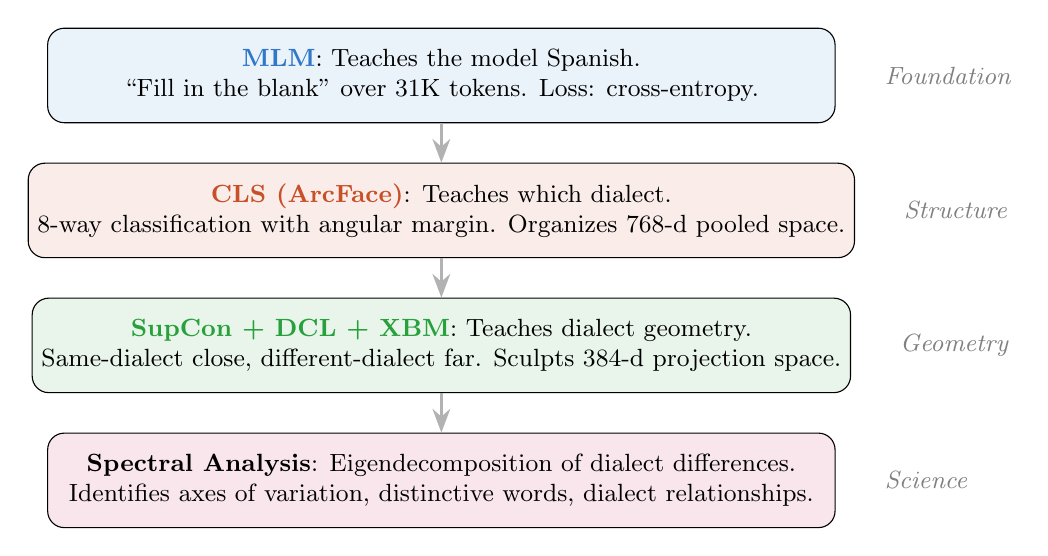
\begin{tikzpicture}[
  box/.style={draw, rounded corners=6pt, minimum width=10cm,
              minimum height=1.2cm, font=\small, align=center},
  arr/.style={-{Stealth[length=3mm]}, very thick, gray!60}
]

\node[box, fill=mlmcolor!10] (mlm) at (0,0)
  {\textcolor{mlmcolor}{\textbf{MLM}}: Teaches the model Spanish.\\
   ``Fill in the blank'' over 31K tokens. Loss: cross-entropy.};

\node[box, fill=clscolor!10, below=0.5cm of mlm] (cls)
  {\textcolor{clscolor}{\textbf{CLS (ArcFace)}}: Teaches which dialect.\\
   8-way classification with angular margin. Organizes 768-d pooled space.};

\node[box, fill=concolor!10, below=0.5cm of cls] (con)
  {\textcolor{concolor}{\textbf{SupCon + DCL + XBM}}: Teaches dialect geometry.\\
   Same-dialect close, different-dialect far. Sculpts 384-d projection space.};

\node[box, fill=purple!10, below=0.5cm of con] (spec)
  {\textbf{Spectral Analysis}: Eigendecomposition of dialect differences.\\
   Identifies axes of variation, distinctive words, dialect relationships.};

\draw[arr] (mlm) -- (cls);
\draw[arr] (cls) -- (con);
\draw[arr] (con) -- (spec);

\node[font=\small\itshape, text=gray, right=0.5cm of mlm]
     {Foundation};
\node[font=\small\itshape, text=gray, right=0.5cm of cls]
     {Structure};
\node[font=\small\itshape, text=gray, right=0.5cm of con]
     {Geometry};
\node[font=\small\itshape, text=gray, right=0.5cm of spec]
     {Science};

\end{tikzpicture}
\end{center}

\bigskip

The EigenDialectos system trains a single neural network with three
simultaneous objectives. MLM builds the language foundation. ArcFace
classification imposes angular dialect structure. Supervised
contrastive learning sculpts the fine-grained geometric relationships
between dialects. The resulting 384-dimensional embeddings are then
analyzed with spectral methods to discover the mathematical structure
of dialectal variation in Spanish.

Every number on the training dashboard---every MLM loss, every CLS
loss, every contrastive loss---is a direct measurement of how well the
model is learning one of these three complementary aspects. When all
three are descending, the system is building a geometric map of
Spanish dialectal space.

\end{document}
